\documentclass[AutoFakeBold,a4paper]{ctexart}
\usepackage{graphicx}
\usepackage{titlesec}
\usepackage{ctex}
\usepackage{xeCJK}
\usepackage{fontspec}
\usepackage{amsmath}
\usepackage{array}
\usepackage{listings}
\usepackage{color, xcolor}
\usepackage{caption}
\usepackage{float}
\usepackage{amsthm,txfonts}
\usepackage{amssymb}
%\usepackage{euler}
\usepackage{fancyhdr}
\usepackage[colorlinks,linkcolor=magenta,citecolor=magenta]{hyperref}
\usepackage{multicol}
\usepackage{titletoc}
\usepackage[biblabel]{cite}
\usepackage[left=1.25in,right=1.25in,top=1in,bottom=1in]{geometry}

\renewcommand\lstlistingname{代码}
%\setCJKmainfont{微软雅黑}[BoldFont=SimHei, ItalicFont=KaiTi]

\pagestyle{fancy}

\fancyhead[RO, RE]{\thepage}
\fancyhead[LO, LE]{\kaishu \leftmark}
\fancyhead[CO, CE]{}

\fancyfoot[RO, RE]{}%lhy1210302421@mail.ustc.edu.cn}
\fancyfoot[LO, LE]{{\kaishu \today}}
\fancyfoot[CO, CE]{}

\setmainfont[Ligatures=TeX]{CMU Serif}
\setsansfont[Ligatures=TeX]{CMU Sans Serif}
\setmonofont[Mapping=]{CMU Typewriter Text}

\setCJKmainfont{PingFangSC-Regular}[BoldFont=PingFangSC-Medium]

\renewcommand{\headrulewidth}{0.1mm} 
\renewcommand{\footrulewidth}{0.1mm}

\lstset{
    basicstyle          =   \sffamily,          % 基本代码风格
    keywordstyle        =   \bfseries,          % 关键字风格
    commentstyle        =   \rmfamily\itshape,  % 注释的风格,斜体
    stringstyle         =   \ttfamily,  % 字符串风格
    flexiblecolumns,                % 别问为什么,加上这个
    numbers             =   left,   % 行号的位置在左边
    showspaces          =   false,  % 是否显示空格,显示了有点乱,所以不现实了
    numberstyle         =   \zihao{-5}\ttfamily,    % 行号的样式,小五号,tt等宽字体
    showstringspaces    =   false,
    captionpos          =   t,      % 这段代码的名字所呈现的位置,t指的是top上面
    frame               =   lrtb,   % 显示边框
    captionpos          =   b       % caption的位置(填t在上,填b在底部)
}

\lstdefinestyle{Python}{
    language        =   Python, % 语言选Python
    basicstyle      =   \zihao{-5}\ttfamily,
    numberstyle     =   \zihao{-5}\ttfamily,
    keywordstyle    =   \color{blue},
    keywordstyle    =   [2] \color{teal},
    stringstyle     =   \color{magenta},
    commentstyle    =   \color[rgb]{0.416,0.6,0.3333}\ttfamily,
    breaklines      =   true,   % 自动换行,建议不要写太长的行
    columns         =   fixed,  % 如果不加这一句,字间距就不固定,很丑,必须加
    basewidth       =   0.5em,
}

\lstdefinestyle{C}{
    language        =   C, % 语言选Python
    basicstyle      =   \zihao{-5}\ttfamily,
    numberstyle     =   \zihao{-5}\ttfamily,
    keywordstyle    =   \color{blue},
    keywordstyle    =   [2] \color{teal},
    stringstyle     =   \color{magenta},
    commentstyle    =   \color[rgb]{0.416,0.6,0.3333}\ttfamily,
    breaklines      =   true,   % 自动换行,建议不要写太长的行
    columns         =   fixed,  % 如果不加这一句,字间距就不固定,很丑,必须加
    basewidth       =   0.5em,
}

\lstdefinestyle{bash}{
    language        =   bash, % 语言选Python
    basicstyle      =   \zihao{-5}\ttfamily,
    numberstyle     =   \zihao{-5}\ttfamily,
    keywordstyle    =   \color{blue},
    keywordstyle    =   [2] \color{teal},
    stringstyle     =   \color{black},
    commentstyle    =   \color[rgb]{0.416,0.6,0.3333}\ttfamily,
    breaklines      =   true,   % 自动换行,建议不要写太长的行
    columns         =   fixed,  % 如果不加这一句,字间距就不固定,很丑,必须加
    basewidth       =   0.5em,
}

% \providecommand{\keywords}[1]{\textbf{\textit{关键字:}} #1}

% \renewcommand{\abstractname}{\textbf{摘要:}}

\begin{document}

\title{\textbf{\Huge 大作业-可行性报告}}

\author{陈思睿 \quad 梁恒宇 \quad 吕泓涛 \quad 汤力宇\\
中国科学技术大学 \quad 安徽合肥}

\date{\today}

\maketitle

\ctexset { section = { format={\Large \bfseries} } }
\ctexset { subsection = { format={\large \bfseries} } }

\titlecontents{section}[2em]{\addvspace{1.3mm}\bf}{%
\contentslabel{2.0em}}{}{\titlerule*[5pt]{$\cdot$}\contentspage}

\titlecontents{subsection}[4.2em]{}{\contentslabel{2.5em}}{}{%
\titlerule*[5pt]{$\cdot$}\contentspage}

\titlecontents{subsubsection}[7.2em]{}{\contentslabel{3.3em}}{}{%
\titlerule*[5pt]{$\cdot$}\contentspage}

\pagenumbering{roman}
\tableofcontents

\pagenumbering{arabic}
\setcounter{page}{1}

% \section{小组成员}

% \begin{itemize}
%     \item 陈思睿
%     \item 梁恒宇
%     \item 吕泓涛
%     \item 汤力宇
% \end{itemize}

\section{项目介绍}

\textbf{使用新兴的eBPF架构,实现兼有安全性和性能的通用沙箱。}

任何操作系统都或多或少的潜藏着安全漏洞,
近年来各大主流OS都被爆出过存在重大安全隐患。
当恶意程序侵入用户的系统,则可能破坏、窃取宝贵的用户数据,
造成不可估量的损失。而为了防止此类事件发生,沙盒技术正在不断发展。
沙盒技术通过对可疑的进程进行隔离与监控,
防止其对系统其它部分造成损害。

然而随着恶意程序的攻击策略不断扩展,
传统沙盒的安全性也难以长期保持,因此一个理想的沙盒应当在高效、
安全同时拥有便于升级维护的特点,这一理想在现有的沙盒中难以实现。
用户态的沙盒存在着大量到内核态的状态切换,带来了严重的性能损失,
而内核态的沙盒则在损失了升级的灵活性的同时带来了更多可能被攻击的安全漏洞。

面对这一困境,本项目希望使用新兴的eBPF架构,
实现一个可以从用户态灵活对其升级的内核态沙盒。
由于BPF架构的设计特征,这一沙盒将不会给内核多带来额外的安全漏洞,
并且将可以实现和内核态相仿的性能。

\section{理论依据}

\subsection{恶意进程}

\subsubsection{linux下的恶意进程}

Linux环境下的经典病毒种类有:\cite{LinuxVirus2020}

\begin{itemize}
    \item BillGates 基于僵尸网络的DDOS攻击
    \item DDG 蠕虫式挖矿
    \item SystemdMiner 蠕虫式挖矿
    \item StartMiner 蠕虫式挖矿
    \item WatchdogsMiner 蠕虫式挖矿
    \item XorDDos 基于僵尸网络的DDOS攻击
    \item RainbowMiner 蠕虫式挖矿
\end{itemize}


\subsubsection{经典攻击方法}

在这篇文章\cite{di2015elf}中介绍了几种经典的恶意进程攻击手段:

\begin{itemize}
    \item 操作系统中的一个用户态组件——动态装载器,
    负责装载二进制文件以及它们依赖的库文件到内存中。
    二进制文件使用动态装载器来支持导入符号的解析功能。有趣的是,
    这恰好就是一个面对加固应用的攻击者通过泄漏库地址与内容尝试“重塑”一个符号的表现。
    windows下的svchost.exe攻击或者linux下的elf攻击都是利用了这个组件进行的攻击。
    \item 早期的栈溢出利用依赖于向缓冲区中注入二进制代码(称为shellcode)的能力,
    并需要覆盖在栈上的一个返回地址使其指向这个缓冲区。随后,当程序从当前函数返回时,
    执行流就会被重定向到攻击者的shellcode,接着攻击者就能取得程序的控制权。
    
\end{itemize}

\subsubsection{恶意进程行为}

卡巴斯基安全实验室在对一个新型zeus变种木马的报告中给出了如下的分析:\cite{ZeuS2018}

\begin{itemize}
    \item 此木马功能非常丰富,包括使用VNC远程桌面控制电脑,截屏并发送,
    读取本地数据并发送,读取用户所有操作并发送,通过注册表开机自动启动,
    监测是否处于沙盒环境并且在沙盒中自动停止活动,监测注册表以防止自己的自动启动被清除。

    \item 此木马的传播主要通过邮件,在恶意邮件中包含一个doc文件作为附件,
    打开后offic会提示需要启用宏来查看完整信息,
    一旦用户点击启用宏后,此木马会自动解码并且将自己复制进svchost.exe
    ,然后其遍可以开始运行各种功能,包括剩余模块的下载,劫持浏览器,窃取本地数据等。
    
    \item 此木马通过读取进程列表以判断是否有正在打开的浏览器,
    然后当存在浏览器的时其会通过浏览器的安全漏洞劫持网页,
    修改用户正在访问的银行网页,截取其输入的密码、账号、pin、等内容并且发送给服务器。
    
    \item 此木马对沙盒有有特殊的监测机制,
    运行在沙盒内的时候系统中会出现若干特征性的监控类设备驱动,
    当发现自己运行在沙盒中时,木马将停止活动以防止自己被安全人员监测出来。
\end{itemize}
此分析给我们带来了如下的提示
\begin{itemize}
    \item 针对某个具体的漏洞来设计沙盒是不切实际的,随着系统体量的膨胀,
    漏洞的存在是不可避免的,至今linux和windows也无法完全杜绝对系统代码的恶意篡改。
    \item 各类资源的隔离对于沙盒的安全性至关重要,必须确保沙盒内的进程只能访问有限的文件服务或者系统服务。
    \item 任何需要与被隔离进程直接交互的服务都有被污染的可能,
    因此多层的隔离或者使用类似于BPF的无法污染的实现方式可以有效的提高对恶意进程的控制力度。
\end{itemize}


\subsection{docker安全}

\begin{enumerate}
    \item 通过namespace,不同docker容器无法访问其他的进程,
    在容器位置向系统请求进程列表会只能看到少数几个局部的容器内进程,无法发现主机的其他进程。
    通过这种技术,类似于zeus的劫持浏览器进程的木马难以危害主机安全。
    
    \item 通过namespace,每个docker会被置入隔离的网络环境中,
    对外的网络功能是通过在每个docker上运行虚拟的网卡并且以桥接模式(默认)与主机网卡链接来实现的。
    在这种情况下可以通过网络安全策略的方式直接控制容器进程的非法网络访问。\\
    \textbf{libnetwork}:docker的网络功能实现的具体技术
    
    \item 利用libcontainer(以及namespace)来实现了对文件系统的保护,
    libcontainer中的chroot技术可以限制某个子系统对应的根目录(rootFS),
    即在容器内的进程来看,当前FS的root就是实际所在的子目录,因而其无法读取或访问主机上的其他文件。
    
    \item cgroup(控制组)是用于限制进程对CPU、内存、网络带宽等运行资源的占用强度的,
    其也可以用来限制容器内程序对设备的访问。不同的进程被组合成一个cgroup,
    作为一个整体参与资源的调度,并且可以通过cgroup组策略来限制当前group可以占用多少资源。
    且cgroup可以嵌套,一个cgroup里面可以包含多个子cgroup。
    如整个docker可能被放在一个cgroup中以限制总资源使用量,
    然后docker里面的每个容器中的进程也各自建立cgroup,
    参与划分docekr-group分配到的总的资源。
    
    \item 联合文件系统(Unionfs),实质上概念很简单,
    此文件系统不管理物理存储,只是依赖于某一个通用的文件系统,
    并且把不同文件夹的内容映射到同一个文件目录内。似乎是docker的重要组成部分。
\end{enumerate}

在这篇文章中,分析了类似于docker的结构的安全性:\cite{bui2015analysis}

\begin{itemize}
    \item 文章基于的模型如下:当hostOS中运行的docker容器中有一部分被恶意进程完全控制了,
    其可以对系统进行如Denial-of-Service 和 Privilege escalation的攻击。
    \item 为了在这种情况下保护系统安全,容器应当做到如下几点:
    \begin{itemize}
        \item process isolation 进程间的隔离
        \item filesystem isolation  文件系统的隔离
        \item device isolation  设备的隔离
        \item IPC isolation 进程间通讯的隔离
        \item network isolation 网络的隔离
        \item limiting of resources 限制资源的使用量
    \end{itemize}
\end{itemize}

对于路线\ref{路线1}或路线\ref{路线3},我们可以参考docker的安全策略,
此策略在各个角度上都有较好的安全性,而且性能相当的高。

\section{技术依据}

\subsection{BPF应用实现}

\subsubsection{一个简单的BPF程序}

运行BPF程序需要两个部分,一个是BPF内核程序,一个是用户态的加载程序。
BPF内核程序需要编译成BPF内核字节码,用户态程序只需要编译成可执行文件。\cite{calavera2019linux}

加载进内核的程序可以使用C代码编写,示例C代码如下:

\lstinputlisting[style=C,caption=BPF内核程序代码]{../LiangHengyu/hello_world/bpf_program.c}

程序被设置为在其他程序开始执行时被调用,并输出“Hello World!”。

它将被编译成字节码:

\lstinputlisting[style=C,caption=BPF字节码]{../LiangHengyu/hello_world/bpf_program_asm.txt}

用户态的加载程序如下,它基本上只起一个加载BPF程序的作用:

\lstinputlisting[style=C,caption=BPF加载程序]{../LiangHengyu/hello_world/loader.c}

执行BPF程序,需要以管理员身份调用该加载程序。程序的执行效果如下图所示:

\begin{figure}[H]
    \centering
    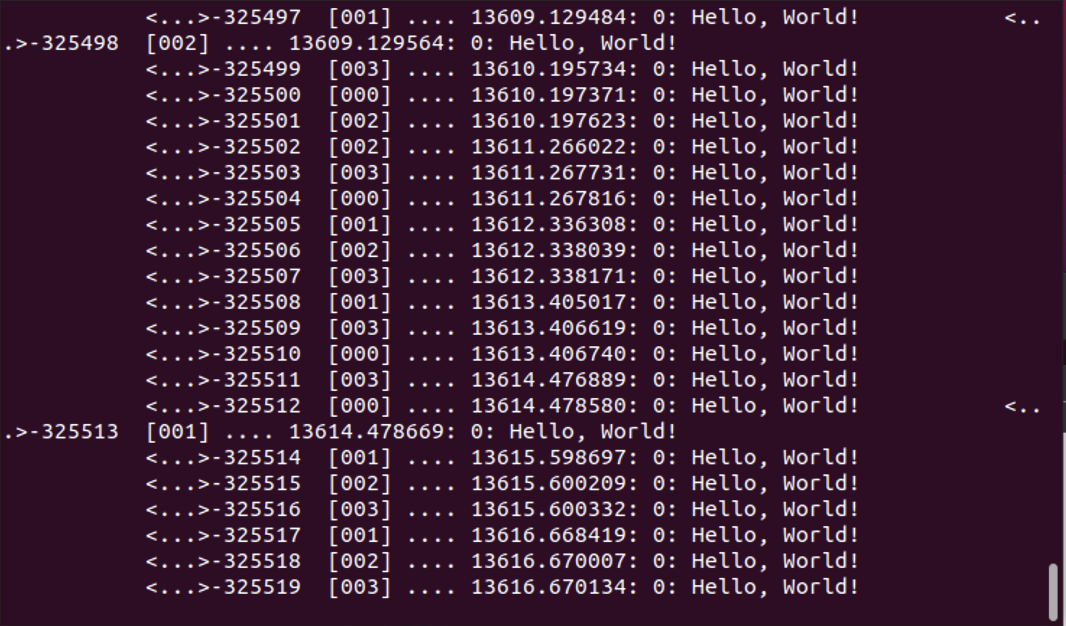
\includegraphics[width=0.7\columnwidth]{../LiangHengyu/hello_world/test1.png}
    \caption{示例程序执行效果}
\end{figure}

可以看到,每当一个系统中有新的程序开始执行时,该BPF程序就会被调用,并输出一个{\ttfamily Hello World!}。

\subsubsection{seccomp实现控制系统调用}

我们编写的seccomp程序实际上是一种“过滤器”,类似“正则表达式”。
它会利用BPF将过滤器程序加载到内核当中监测被监控程序的系统调用,
一旦该程序的系统调用匹配上了你编写的格式,对该被监控程序的一些行为就会被触发。

seccomp在头文件{\ttfamily <linux/seccomp.h>}中定义了有限的一些控制被监控的进程的操作。

\lstinputlisting[style=C,caption=seccomp头文件]{../LiangHengyu/seccomp/seccomp_part.h}

例如,使用{\ttfamily SECCOMP\_RET\_KILL\_PROCESS}会关闭该程序,
使用{\ttfamily SECCOMP\_RET\_ERRNO}会拒绝该程序相关的系统调用。

这里有如下的一个示例程序,这个程序会拒绝被调用程序的所有和写相关的系统调用。

\lstinputlisting[style=C,caption=BPF加载程序]{../LiangHengyu/seccomp/main.c}

编译好这个程序,我们使用这个程序调用一个需要进行写操作的程序{\ttfamily ls},
同时我们还需要使用{\ttfamily strace}来跟踪{\ttfamily ls}所有的系统调用。
执行的\textbf{部分}结果如下:

\lstinputlisting[style=bash,caption=seccomp程序执行结果]{../LiangHengyu/seccompshort.txt}

为了节省空间,大部分程序的输出都被省略掉了,完整结果可见代码\ref{seccomp完整}。

可以看到,{\ttfamily ls}正确执行出了通常的运行结果:
{\ttfamily "total 32\verb|\|ndrwxrwxr-x 2 lhy lhy 40"},
但是执行的{\ttfamily write}系统调用均被拒绝了,所以在终端并不会看到任何的输出。
此外,程序并没有被kill掉,调用了不允许的系统调用后,还在正常运行。

\subsubsection{小结}

BPF程序能高效成为一个内核中的profiler,这是我们接下来将引出的第\ref{路线1}和第\ref{路线3}的主要技术依据,
在后文中会对技术依据进行更详细的解释。

但是我们也能注意到,类似seccomp的BPF安全应用有非常大的局限性。
如果我们的过滤机制不够完善,它在阻止病毒程序的运行的同时,还阻止了正常程序的运行。
这也是我们改进想法由来的原因之一,同时,我们据此还有了另一个思路。
下一小节中我们会尝试解除当前BPF的一些限制,让BPF有更完善的功能,支持我们沙盒的运行。

\subsection{Linux内核BPF源码的调研}
路线一或者路线二中希望实现的沙盒程序的复杂度可能难以直接载入现有的linux eBPF,
为了实现这些功能,我们将有必要对linux的eBPF代码进行修改或者需要定制自己的eBPF内核模块。
为此,我们对linux内核中的BPF源码进行了简单的调研。具体的,我们研究了如何修改verify模块,
如何添加更多的helper函数,
\subsubsection{修改linux中BPF源码的意义}
BPF的程序的功能丰富度是和内核对BPF程序的支持直接相关的,
例如每个BPF程序的输入输出规范都是直接以模板形式定义在内核源码中的,
而BPF程序可以使用的系统调用也是直接在linux/kernel/bpf/helper.c中直接定义的,
因此实现诸如劫持系统调用等的功能讲不可避免的会涉及到对内核中BPF源码的修改或重写。
我们也有可能会在后续的工作中发现我们的程序在现有的verifier体系下难以得到认可,
例如我们在bpf中实现的文件系统管理服务可能会被verifier认定为不会终止,于是被拒绝载入到内核中,
这种情况下我们便会需要修改verifier对软件安全性的认证过程,用更加智能的检测手段来检查bpf程序的安全性,
从而防止我们的程序被错误的认定为不安全。
\subsubsection{linux下BPF verifier部分的源码结构分析}
与linux中大部分源码相似,BPFverifier的头文件位于linux/include/linux/bpf_verifier.h,
原文件位于linux/kernel/bpf/verifier.c。头文件中最重要的数据结构为struct bpf_verifier_env,
这个数据结构作为verify过程中最核心的结构出现在了源文件相关函数中。此数据结构中包括了程序源码,各个验证流程的状态(通过与否)等,
后文中的check函数中主要通过传递env变量来进行各级的验证流。而原文件中最重要的函数为bpf_chekc(),
承载了验证bpf安全性的主要功能,包括代码的载入,对代码规模、运行路线、最坏运行时间的分析等各项检查分别在此函数中被调用。
其中涉及到的最大代码长度、最长运行时间等重要常数通过宏定义的方式定义在此文件或bpf.c中。
\begin{figure}[H]
    \centering
    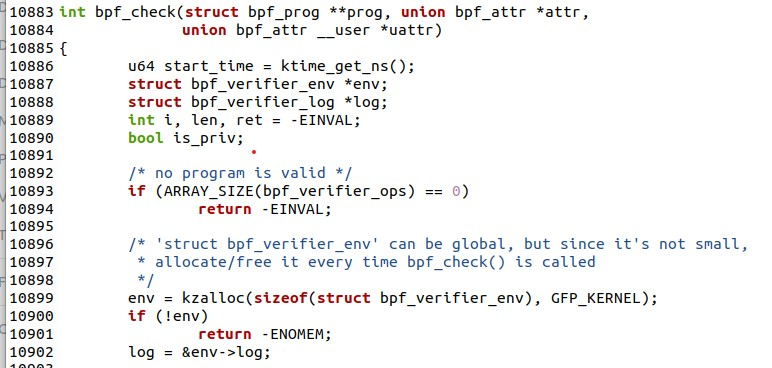
\includegraphics[width=0.7\columnwidth]{../LvHongtao/pic_2.jpg}
    \caption{bpf_check函数}
\end{figure}

\subsubsection{linux下BPF helper函数与BPF program type的相关分析}
linux下有关helper函数的主要定义都位于linux/kernel/bpf/helpers.c中,其中对helper函数的格式、类型以及具体的实例有着详细的定义。
我们在这段源码中发现了诸如__bpf_spin_lock,和mmap抽象存储相关的各种helper函数的具体实现,在后续的工作中,
我们可以直接将我们需要的helper函数添加在此处来实现我们需要的功能。\\ 
而有关BPF program type的主要代码都位于linux/include/bpf_types.h中,
其中定义了常用的诸如BPF_PROG_TYPE_SOCKET_FILTER,BPF_PROG_TYPE_XDP等BPF程序及其相关输入输出参数类型,
这些程序类型的声明方式对我们的代码编写有着重要的指导意义。
\begin{figure}[H]
    \centering
    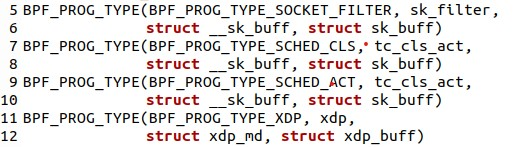
\includegraphics[width=0.7\columnwidth]{../LvHongtao/pic_3.jpg}
    \caption{bpf_types.h}
\end{figure}

\subsubsection{对内核代码的重编译和加载}
与一般的模块化加载方式不同,bpf相关代码只能在编译之初就集成于内核中,因此修改BPF源码后,
有必要对内核进行整体重新编译。linux对内核更新的支持非常友好,其允许用户在系统中完成新内核的编译和加载,
然后直接通过重启以切换到新内核。具体的,完成源码的修改后,通过正常的编译指令可以将内核编译完成,依次完成新版本模块的装载和新版本内核的装载后,
完成boot目录下grub文件的修改,最后通过reboot重启以进入新版本的内核。




\section{技术路线}
在现阶段,我们提出了三种具体的实现本项目的路线。
\subsection{路线一:轻量化bpf沙盒实现方案}
这一路线中,我们希望借鉴docker的隔离结构,尽可能使沙盒本体实现轻量化和高效。
这一路线中,bpf的运行模式与seccomp中拦截系统调用的做法类似,举例来说我们可以通过使bpf程序拦截用户进程的文件类系统调用,
将其中的具体目录信息篡改后转发给系统,如将用户进程请求的read C:/root/的访问请求拦截篡改为D:/user/sandbox/ins1/C/root来进行实际的执行,
通过这种手段可以实现docekr中的fakeroot技术。
我们希望使用类似的方式在bpf环境下实现docker engine中的各项隔离技术,以实现和docker同等的隔离性,并且可以有望实现更高的安全性和性能。
优点:实现较为简单,沙盒本体较为轻量化。
缺点:沙盒层数较少,故一旦被恶意进程攻破会存在着危害主机系统的可能。

\subsection{路线二:bpf内实现进程虚拟化}
这一路线中,我们希望借鉴gVisor的多层沙盒结构,尽可能使沙盒本体实现最大化的安全性和相对gVisor更高的运行效率
gVisor维护了一套虚拟化的内核服务,例如沙盒内的局部文件系统。这种结构设计比路线一可以实现更好的安全性,
恶意进程将难以同时捕捉到局部文件系统和主机文件系统的漏洞,从而增大其污染主机系统的难度。
本路线中我们希望在bpf中实现局部的文件系统或局部的动态装载器等系统服务,这种方式能够实现更加完备的隔离性,减少沙盒与主机系统的实际交互。
使用bpf结构可以比gvisor更加容易和高效的捕捉拦截转发沙盒进程的系统调用,同时bpf结构几乎没有被篡改代码内容的危险,
从而实现了比gvisor更进一步的安全性。
优点:最大化的安全性,比gVisor等同类原理沙盒更高的效率。
缺点:体量较大,实现复杂度高。

\subsection{路线三:bpf优化用户态沙盒}
这一路线为备选路线,当对内核bpf模块修改失败后会转为使用此路线。
这一路线依据于gVisor等用户态沙盒会在劫持系统调用过程中损失大量的性能这一特征。BPF可以作为优秀的监控拦截模块,
使用现有的BPF框架即可高效简单的实现gVisor中需要的劫持系统调用这一步骤,可以同时优化gVisor的性能与安全性,
选择此路线时我们将选择某个现有的用户态沙盒应用,着手使用bpf结构优化其中的部分功能。
优点:代码难度较低。
缺点:相较现有的成熟解决方案缺少突破性的创新,无法做到根本性的优化。




\bibliography{../paper.bib}
\bibliographystyle{ieeetr}

\section{附录}

\subsection{seccomp完整输出结果}

\lstinputlisting[style=bash,caption=seccomp程序执行结果,label=seccomp完整]{../LiangHengyu/seccompout.txt}

\end{document}